% Created by tikzDevice version 0.6.2-92-0ad2792 on 2012-12-03 17:29:26
% !TEX encoding = UTF-8 Unicode
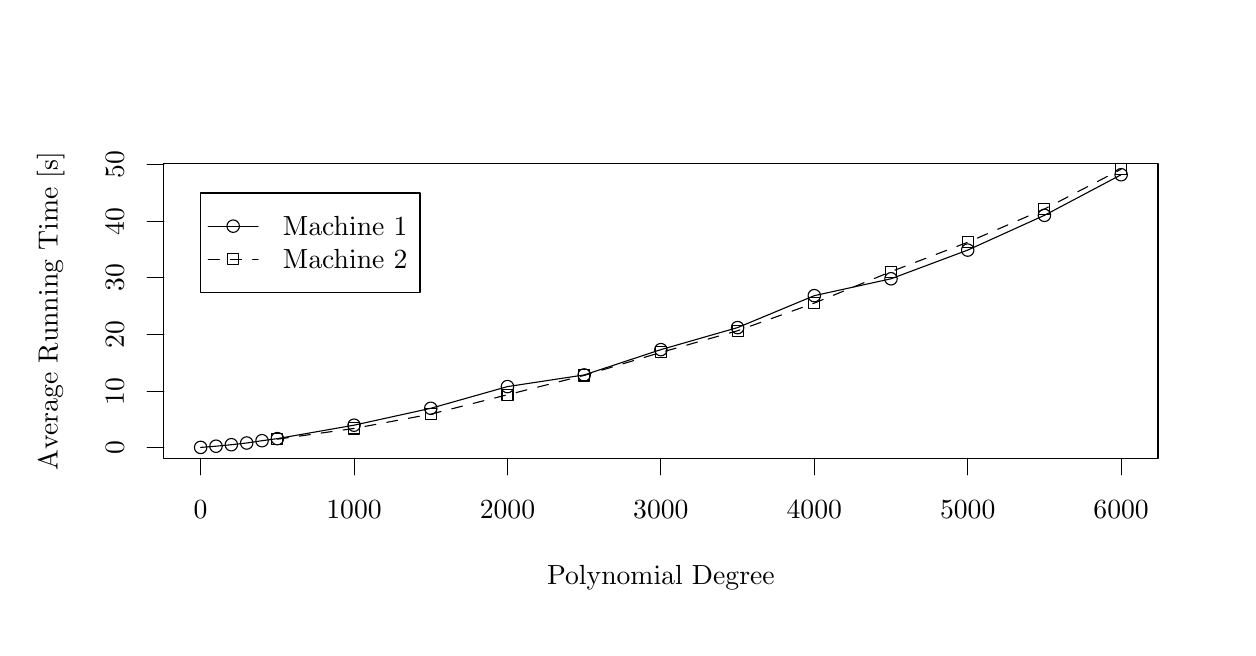
\begin{tikzpicture}[x=1pt,y=1pt]
\definecolor[named]{fillColor}{rgb}{1.00,1.00,1.00}
\path[use as bounding box,fill=fillColor,fill opacity=0.00] (0,0) rectangle (433.62,216.81);
\begin{scope}
\path[clip] ( 49.20, 61.20) rectangle (408.42,167.61);
\definecolor[named]{drawColor}{rgb}{0.00,0.00,0.00}

\path[draw=drawColor,line width= 0.4pt,line join=round,line cap=round] ( 62.50, 65.14) --
	( 68.05, 65.57) --
	( 73.59, 66.11) --
	( 79.14, 66.73) --
	( 84.68, 67.56) --
	( 90.22, 68.31) --
	(117.94, 73.17) --
	(145.66, 79.27) --
	(173.37, 87.11) --
	(201.09, 91.32) --
	(228.81,100.47) --
	(256.53,108.43) --
	(284.25,119.97) --
	(311.96,126.07) --
	(339.68,136.44) --
	(367.40,149.00) --
	(395.12,163.67);

\path[draw=drawColor,line width= 0.4pt,line join=round,line cap=round] ( 62.50, 65.14) circle (  2.25);

\path[draw=drawColor,line width= 0.4pt,line join=round,line cap=round] ( 68.05, 65.57) circle (  2.25);

\path[draw=drawColor,line width= 0.4pt,line join=round,line cap=round] ( 73.59, 66.11) circle (  2.25);

\path[draw=drawColor,line width= 0.4pt,line join=round,line cap=round] ( 79.14, 66.73) circle (  2.25);

\path[draw=drawColor,line width= 0.4pt,line join=round,line cap=round] ( 84.68, 67.56) circle (  2.25);

\path[draw=drawColor,line width= 0.4pt,line join=round,line cap=round] ( 90.22, 68.31) circle (  2.25);

\path[draw=drawColor,line width= 0.4pt,line join=round,line cap=round] (117.94, 73.17) circle (  2.25);

\path[draw=drawColor,line width= 0.4pt,line join=round,line cap=round] (145.66, 79.27) circle (  2.25);

\path[draw=drawColor,line width= 0.4pt,line join=round,line cap=round] (173.37, 87.11) circle (  2.25);

\path[draw=drawColor,line width= 0.4pt,line join=round,line cap=round] (201.09, 91.32) circle (  2.25);

\path[draw=drawColor,line width= 0.4pt,line join=round,line cap=round] (228.81,100.47) circle (  2.25);

\path[draw=drawColor,line width= 0.4pt,line join=round,line cap=round] (256.53,108.43) circle (  2.25);

\path[draw=drawColor,line width= 0.4pt,line join=round,line cap=round] (284.25,119.97) circle (  2.25);

\path[draw=drawColor,line width= 0.4pt,line join=round,line cap=round] (311.96,126.07) circle (  2.25);

\path[draw=drawColor,line width= 0.4pt,line join=round,line cap=round] (339.68,136.44) circle (  2.25);

\path[draw=drawColor,line width= 0.4pt,line join=round,line cap=round] (367.40,149.00) circle (  2.25);

\path[draw=drawColor,line width= 0.4pt,line join=round,line cap=round] (395.12,163.67) circle (  2.25);
\end{scope}
\begin{scope}
\path[clip] (  0.00,  0.00) rectangle (433.62,216.81);
\definecolor[named]{drawColor}{rgb}{0.00,0.00,0.00}

\path[draw=drawColor,line width= 0.4pt,line join=round,line cap=round] ( 62.50, 61.20) -- (395.12, 61.20);

\path[draw=drawColor,line width= 0.4pt,line join=round,line cap=round] ( 62.50, 61.20) -- ( 62.50, 55.20);

\path[draw=drawColor,line width= 0.4pt,line join=round,line cap=round] (117.94, 61.20) -- (117.94, 55.20);

\path[draw=drawColor,line width= 0.4pt,line join=round,line cap=round] (173.37, 61.20) -- (173.37, 55.20);

\path[draw=drawColor,line width= 0.4pt,line join=round,line cap=round] (228.81, 61.20) -- (228.81, 55.20);

\path[draw=drawColor,line width= 0.4pt,line join=round,line cap=round] (284.25, 61.20) -- (284.25, 55.20);

\path[draw=drawColor,line width= 0.4pt,line join=round,line cap=round] (339.68, 61.20) -- (339.68, 55.20);

\path[draw=drawColor,line width= 0.4pt,line join=round,line cap=round] (395.12, 61.20) -- (395.12, 55.20);

\node[text=drawColor,anchor=base,inner sep=0pt, outer sep=0pt, scale=  1.00] at ( 62.50, 39.60) {0};

\node[text=drawColor,anchor=base,inner sep=0pt, outer sep=0pt, scale=  1.00] at (117.94, 39.60) {1000};

\node[text=drawColor,anchor=base,inner sep=0pt, outer sep=0pt, scale=  1.00] at (173.37, 39.60) {2000};

\node[text=drawColor,anchor=base,inner sep=0pt, outer sep=0pt, scale=  1.00] at (228.81, 39.60) {3000};

\node[text=drawColor,anchor=base,inner sep=0pt, outer sep=0pt, scale=  1.00] at (284.25, 39.60) {4000};

\node[text=drawColor,anchor=base,inner sep=0pt, outer sep=0pt, scale=  1.00] at (339.68, 39.60) {5000};

\node[text=drawColor,anchor=base,inner sep=0pt, outer sep=0pt, scale=  1.00] at (395.12, 39.60) {6000};

\path[draw=drawColor,line width= 0.4pt,line join=round,line cap=round] ( 49.20, 65.00) -- ( 49.20,167.31);

\path[draw=drawColor,line width= 0.4pt,line join=round,line cap=round] ( 49.20, 65.00) -- ( 43.20, 65.00);

\path[draw=drawColor,line width= 0.4pt,line join=round,line cap=round] ( 49.20, 85.46) -- ( 43.20, 85.46);

\path[draw=drawColor,line width= 0.4pt,line join=round,line cap=round] ( 49.20,105.92) -- ( 43.20,105.92);

\path[draw=drawColor,line width= 0.4pt,line join=round,line cap=round] ( 49.20,126.39) -- ( 43.20,126.39);

\path[draw=drawColor,line width= 0.4pt,line join=round,line cap=round] ( 49.20,146.85) -- ( 43.20,146.85);

\path[draw=drawColor,line width= 0.4pt,line join=round,line cap=round] ( 49.20,167.31) -- ( 43.20,167.31);

\node[text=drawColor,rotate= 90.00,anchor=base,inner sep=0pt, outer sep=0pt, scale=  1.00] at ( 34.80, 65.00) {0};

\node[text=drawColor,rotate= 90.00,anchor=base,inner sep=0pt, outer sep=0pt, scale=  1.00] at ( 34.80, 85.46) {10};

\node[text=drawColor,rotate= 90.00,anchor=base,inner sep=0pt, outer sep=0pt, scale=  1.00] at ( 34.80,105.92) {20};

\node[text=drawColor,rotate= 90.00,anchor=base,inner sep=0pt, outer sep=0pt, scale=  1.00] at ( 34.80,126.39) {30};

\node[text=drawColor,rotate= 90.00,anchor=base,inner sep=0pt, outer sep=0pt, scale=  1.00] at ( 34.80,146.85) {40};

\node[text=drawColor,rotate= 90.00,anchor=base,inner sep=0pt, outer sep=0pt, scale=  1.00] at ( 34.80,167.31) {50};

\path[draw=drawColor,line width= 0.4pt,line join=round,line cap=round] ( 49.20, 61.20) --
	(408.42, 61.20) --
	(408.42,167.61) --
	( 49.20,167.61) --
	( 49.20, 61.20);
\end{scope}
\begin{scope}
\path[clip] (  0.00,  0.00) rectangle (433.62,216.81);
\definecolor[named]{drawColor}{rgb}{0.00,0.00,0.00}

\node[text=drawColor,anchor=base,inner sep=0pt, outer sep=0pt, scale=  1.00] at (228.81, 15.60) {Polynomial Degree};

\node[text=drawColor,rotate= 90.00,anchor=base,inner sep=0pt, outer sep=0pt, scale=  1.00] at ( 10.80,114.41) {Average Running Time [s]};
\end{scope}
\begin{scope}
\path[clip] ( 49.20, 61.20) rectangle (408.42,167.61);
\definecolor[named]{drawColor}{rgb}{0.00,0.00,0.00}

\path[draw=drawColor,line width= 0.4pt,dash pattern=on 4pt off 4pt ,line join=round,line cap=round] ( 90.22, 68.11) --
	(117.94, 71.99) --
	(145.66, 77.16) --
	(173.37, 84.17) --
	(201.09, 91.15) --
	(228.81, 99.46) --
	(256.53,107.30) --
	(284.25,117.28) --
	(311.96,128.65) --
	(339.68,139.27) --
	(367.40,151.26) --
	(395.12,165.65);

\path[draw=drawColor,line width= 0.4pt,line join=round,line cap=round] ( 88.23, 66.12) rectangle ( 92.22, 70.11);

\path[draw=drawColor,line width= 0.4pt,line join=round,line cap=round] (115.95, 69.99) rectangle (119.93, 73.98);

\path[draw=drawColor,line width= 0.4pt,line join=round,line cap=round] (143.66, 75.16) rectangle (147.65, 79.15);

\path[draw=drawColor,line width= 0.4pt,line join=round,line cap=round] (171.38, 82.18) rectangle (175.37, 86.16);

\path[draw=drawColor,line width= 0.4pt,line join=round,line cap=round] (199.10, 89.15) rectangle (203.09, 93.14);

\path[draw=drawColor,line width= 0.4pt,line join=round,line cap=round] (226.82, 97.47) rectangle (230.80,101.46);

\path[draw=drawColor,line width= 0.4pt,line join=round,line cap=round] (254.53,105.30) rectangle (258.52,109.29);

\path[draw=drawColor,line width= 0.4pt,line join=round,line cap=round] (282.25,115.28) rectangle (286.24,119.27);

\path[draw=drawColor,line width= 0.4pt,line join=round,line cap=round] (309.97,126.66) rectangle (313.96,130.65);

\path[draw=drawColor,line width= 0.4pt,line join=round,line cap=round] (337.69,137.28) rectangle (341.67,141.26);

\path[draw=drawColor,line width= 0.4pt,line join=round,line cap=round] (365.40,149.26) rectangle (369.39,153.25);

\path[draw=drawColor,line width= 0.4pt,line join=round,line cap=round] (393.12,163.66) rectangle (397.11,167.65);

\path[draw=drawColor,line width= 0.4pt,line join=round,line cap=round] ( 62.56,157.08) rectangle (141.75,121.08);

\path[draw=drawColor,line width= 0.4pt,line join=round,line cap=round] ( 65.26,145.08) -- ( 83.26,145.08);

\path[draw=drawColor,line width= 0.4pt,dash pattern=on 4pt off 4pt ,line join=round,line cap=round] ( 65.26,133.08) -- ( 83.26,133.08);

\path[draw=drawColor,line width= 0.4pt,line join=round,line cap=round] ( 74.26,145.08) circle (  2.25);

\path[draw=drawColor,line width= 0.4pt,line join=round,line cap=round] ( 72.27,131.08) rectangle ( 76.25,135.07);

\node[text=drawColor,anchor=base west,inner sep=0pt, outer sep=0pt, scale=  1.00] at ( 92.26,141.63) {Machine 1  };

\node[text=drawColor,anchor=base west,inner sep=0pt, outer sep=0pt, scale=  1.00] at ( 92.26,129.63) {Machine 2  };
\end{scope}
\end{tikzpicture}
